\documentclass[t,aspectratio=169]{beamer} % 使用16:9宽高比
\usetheme{Madrid} % 选择Madrid主题
\usecolortheme{default} % 使用默认颜色主题

% 设置字体
\usepackage[UTF8]{ctex}
\usefonttheme{structurebold} % 加粗结构字体

% 数学包
\usepackage{amsmath, amssymb, bm}
\usepackage{url}
\usepackage{booktabs}

% 图形包
\usepackage{graphicx}

% 标题页信息
\title[10.3.可视化CNN]{第10章：卷积网络}
\subtitle{第3节：可视化训练好的CNN (Visualizing Trained CNNs)}
\author{《深度学习基础》课程小组}
% \institute{上海立信会计金融学院}
\date{\today}

\begin{document}

% 标题页
\frame{\titlepage}

% 目录页
\begin{frame}
    \frametitle{目录}
    \tableofcontents
\end{frame}

% ============================================================
% 第一部分：视觉皮层
% ============================================================
\section{视觉皮层}

\begin{frame}
    \frametitle{1. 视觉皮层 (10.3.1)}
    \begin{itemize}
        \item CNN 的许多动机来自\alert{神经科学}的开创性研究。
        \item 视网膜电信号通过视觉皮层的一系列处理层变换。
        \item 视觉皮层位于大脑后部，神经元组织成\alert{二维薄片}，形成对二维视野的映射。
        \item \textbf{Hubel 和 Wiesel (1959)}：测量猫视觉皮层单个神经元的电响应。
        \begin{itemize}
            \item \alert{简单细胞}：对特定角度、特定位置的简单边缘有强烈响应。
            \item \alert{复杂细胞}：对更复杂刺激响应，似乎由简单细胞输出组合而来。
            \item 更深层：更特定的响应，更大的不变性（“祖母细胞”）。
        \end{itemize}
    \end{itemize}
\end{frame}

\begin{frame}[allowframebreaks]
    \frametitle{1.1 Gabor 滤波器}
    简单细胞的响应可用 \alert{Gabor 滤波器}建模：
    \begin{equation}
        G(x, y) = A \exp\left(-\alpha \overline{x}^2 - \beta \overline{y}^2\right) \sin\left(\omega \overline{x} + \phi\right)
        \tag{10.6}
    \end{equation}
    其中
    \begin{align}
        \overline{x} &= (x - x_0) \cos(\theta) + (y - y_0) \sin(\theta) \tag{10.7} \\
        \overline{y} &= -(x - x_0) \sin(\theta) + (y - y_0) \cos(\theta) \tag{10.8}
    \end{align}
    \begin{itemize}
        \item $\theta$：\alert{方向角}
        \item $\omega$：\alert{频率}，$\phi$：\alert{相位角}
        \item $(x_0, y_0)$：\alert{位置}
        \item $\alpha, \beta$：\alert{衰减速率}（控制局部化范围）
    \end{itemize}
    \begin{figure}
        \centering
        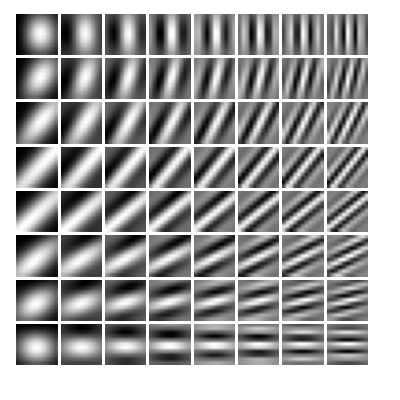
\includegraphics[width=0.25\textwidth]{ch10-3-1/figure-10-11.png}
        \caption{Gabor 滤波器示例：$\theta$ 从 $0$ 到 $\pi/2$，$\omega$ 从 1 到 10。}
    \end{figure}
\end{frame}

\begin{frame}
    \frametitle{1.2 复杂细胞与 Neocognitron}
    \begin{itemize}
        \item \alert{复杂细胞}：组合简单细胞输出，对位置等小变化有\alert{不变性}。
        \begin{itemize}
            \item 类似 CNN 中的\alert{池化单元}。
        \end{itemize}
        \item 更深层：更具体的响应，更大的不变性。
        \item \alert{Neocognitron} (Fukushima, 1980)：CNN 的前身。
        \begin{itemize}
            \item 多层处理：局部感受野 + 共享权重
            \item 局部平均/最大池化 $\Rightarrow$ 位置不变性
            \item \textbf{局限}：缺乏端到端训练（早于反向传播）
            \item 依赖无监督聚类算法的\alert{贪婪逐层学习}
        \end{itemize}
    \end{itemize}
\end{frame}

% ============================================================
% 第二部分：可视化训练好的滤波器
% ============================================================
\section{可视化训练好的滤波器}

\begin{frame}
    \frametitle{2. 可视化训练好的滤波器 (10.3.2)}
    \begin{itemize}
        \item \textbf{第一层滤波器}：可直接可视化为小图像。
        \begin{itemize}
            \item 对应原始输入图像空间中的小图像块。
            \item 第一层计算滤波器与图像块的\alert{内积}。
            \item 内积幅度大 $\Rightarrow$ 单元激活强。
        \end{itemize}
        \item 图 10.12：ImageNet 训练的 AlexNet 第一层滤波器。
        \begin{itemize}
            \item 与 Gabor 滤波器\alert{显著相似}。
        \end{itemize}
        \item \textbf{但注意}：这不意味着 CNN 是大脑工作方式的良好模型。
        \begin{itemize}
            \item 类似结果也可由多种统计方法得到。
            \item 这些滤波器是\alert{自然图像统计的一般性质}。
        \end{itemize}
    \end{itemize}
\end{frame}

\begin{frame}
    \frametitle{2.1 后续层的可视化}
    \begin{itemize}
        \item 后续层\alert{难以直接解释}：输入不是图像块，而是滤波器响应的组合。
        \item \textbf{方法}（类似 Hubel 和 Wiesel）：
        \begin{itemize}
            \item 向网络呈现大量图像块
            \item 观察哪些产生最高激活值
        \end{itemize}
    \end{itemize}
    \begin{block}{图 10.13 的发现：层次结构}
        \begin{itemize}
            \item 第 1 层：\alert{边缘}
            \item 第 2 层：\alert{纹理和简单形状}
            \item 第 3 层：\alert{物体部件}（如车轮）
            \item 第 5 层：\alert{完整物体}
        \end{itemize}
    \end{block}
\end{frame}

\begin{frame}
    \frametitle{2.2 数值优化生成代表性图像}
    \begin{itemize}
        \item 扩展技术：对输入变量进行\alert{数值优化}，最大化特定单元的激活。
        \item 若选择输出单元，可寻找最能代表对应类别的图像。
        \item \textbf{关键技巧}：最大化\alert{预激活值}（softmax 之前）而非类别概率。
        \begin{itemize}
            \item softmax 分母会耦合其他类别。
            \item 例：优化“狗”的 softmax 输出可能使图像“不那么像猫”。
        \end{itemize}
        \item \textbf{需要正则化}：
        \begin{itemize}
            \item 无约束优化 $\Rightarrow$ 像素值趋向无穷大 + 高频结构
            \item Yosinski et al. (2015)：像素平方和 + 模糊 + 裁剪
        \end{itemize}
    \end{itemize}
    \begin{figure}
        \centering
        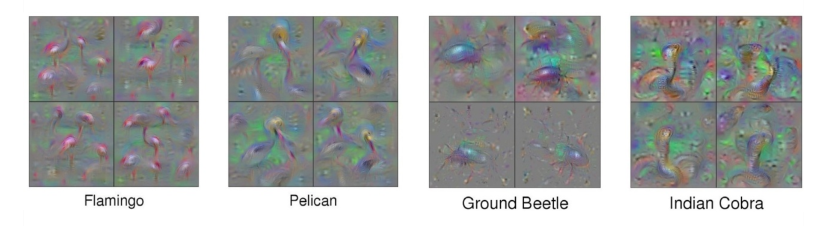
\includegraphics[width=0.4\textwidth]{ch10-3-2/figure-10-14.png}
        \caption{通过最大化类别概率生成的合成图像。}
    \end{figure}
\end{frame}

% ============================================================
% 第三部分：显著图
% ============================================================
\section{显著图}

\begin{frame}[allowframebreaks]
    \frametitle{3. 显著图 (10.3.3)}
    \begin{itemize}
        \item \alert{显著图}：识别图像中对确定类别标签\alert{最重要的区域}。
        \item \textbf{选择最后一个卷积层的原因}：
        \begin{itemize}
            \item 仍保留\alert{空间定位}信息
            \item 具有\alert{最高层次的语义}表示
            \item 后续全连接层会丢失空间信息
        \end{itemize}
        \item \alert{Grad-CAM}（梯度类别激活映射）方法：
    \end{itemize}
    \begin{block}{Grad-CAM 核心步骤}
        \begin{enumerate}
            \item 计算类别 $c$ 的预激活值 $a^{(c)}$ 对最后卷积层各单元 $a_{ij}^{(k)}$ 的导数
            \item 对每个通道取平均，得到权重：
            \begin{equation}
                \alpha_k = \frac{1}{M_k} \sum_i \sum_j \frac{\partial a^{(c)}}{\partial a_{ij}^{(k)}}
                \tag{10.9}
            \end{equation}
            \item 加权求和：
            \begin{equation}
                \mathbf{L} = \sum_k \alpha_k \mathbf{A}^{(k)}
                \tag{10.10}
            \end{equation}
        \end{enumerate}
    \end{block}
    \begin{itemize}
        \item 显著图与最后卷积层同维度（如 VGG 为 $14 \times 14$），可叠加为热力图。
    \end{itemize}
\end{frame}

% ============================================================
% 第四部分：对抗攻击
% ============================================================
\section{对抗攻击}

\begin{frame}[allowframebreaks]
    \frametitle{4. 对抗攻击 (10.3.4)}
    \begin{itemize}
        \item \alert{对抗攻击}：对图像进行微小、人类不可察觉的修改，使网络错误分类。
        \item \alert{快速梯度符号法} (Goodfellow et al., 2014)：
        \begin{equation}
            \mathbf{x}' = \mathbf{x} + \epsilon \operatorname{sign}(\nabla_{\mathbf{x}} E(\mathbf{x}, t))
            \tag{10.11}
        \end{equation}
        \begin{itemize}
            \item $t$：真实标签
            \item $E(\mathbf{x}, t)$：误差函数（如负对数似然）
            \item 梯度用\alert{反向传播}高效计算
        \end{itemize}
        \item \textbf{与训练的区别}：
        \begin{itemize}
            \item 训练：调整\alert{网络参数}以\alert{最小化}误差
            \item 攻击：固定网络参数，调整\alert{图像}以\alert{最大化}误差
        \end{itemize}
        \item $\epsilon$ 小 $\Rightarrow$ 人类不可察觉，但网络可能高置信度误分类。
    \end{itemize}
    \begin{figure}
        \centering
        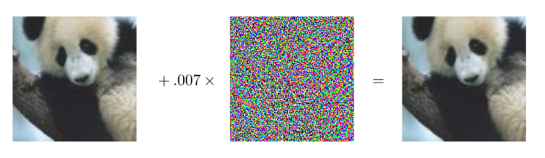
\includegraphics[width=0.5\textwidth]{ch10-3-4/figure-10-16.png}
        \caption{对抗攻击示例：熊猫 $\to$ 长臂猿（99.3\% 置信度）。}
    \end{figure}
\end{frame}

\begin{frame}[allowframebreaks]
    \frametitle{4.1 对抗攻击的普遍性与安全影响}
    \begin{itemize}
        \item 表面看似过拟合，但事实并非如此：
        \begin{itemize}
            \item 对抗图像可\alert{迁移}：欺骗多个不同网络。
            \item \alert{线性模型}也能产生类似对抗结果。
            \item 可构造\alert{物理制品}，使真实拍摄图像被误分类。
        \end{itemize}
        \item \textbf{安全影响}：
        \begin{itemize}
            \item 为攻击训练好的分类器创造机会。
            \item 简单修改训练过程可应对基本攻击。
            \item 更复杂方法难以防御，仍是\alert{开放研究领域}。
        \end{itemize}
    \end{itemize}
    \begin{figure}
        \centering
        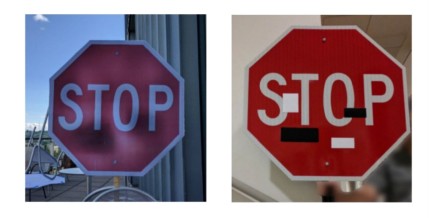
\includegraphics[width=0.35\textwidth]{ch10-3-4/figure-10-17.png}
        \caption{修改后的停车标志被分类为限速标志。}
    \end{figure}
\end{frame}

% ============================================================
% 第五部分：合成图像
% ============================================================
\section{合成图像}

\begin{frame}
    \frametitle{5. DeepDream：合成图像 (10.3.5)}
    \begin{itemize}
        \item 目标：生成具有\alert{夸张特征}的合成图像。
        \item 确定特定隐藏层中哪些节点响应强烈，然后修改图像以\alert{放大这些响应}。
    \end{itemize}
    \begin{block}{DeepDream 基本步骤}
        \begin{enumerate}
            \item 图像输入网络，前向传播到某个特定层
            \item 将该层的反向传播 $\delta$ 变量设为该层节点的\alert{预激活值}
            \item 反向传播到输入层，得到像素上的\alert{梯度向量}
            \item 沿梯度方向迈出一小步修改图像
            \item 可重复多次以获得更强增强
        \end{enumerate}
    \end{block}
    \begin{itemize}
        \item 目标函数：
        \begin{equation}
            F(\mathbf{I}) = \sum_{i,j,k} a_{ijk}(\mathbf{I})^2
            \tag{10.12}
        \end{equation}
        \item 正则化：\alert{空间平滑} + \alert{像素裁剪}，避免高频结构。
    \end{itemize}
\end{frame}

\begin{frame}
    \frametitle{5.1 DeepDream 的效果与用途}
    \begin{itemize}
        \item 可应用于照片，或从\alert{随机噪声}开始生成完全由网络生成的图像。
        \item 有趣：尽管 CNN 被训练用于\alert{区分}物体类别，它们似乎捕捉了\alert{生成}图像所需的部分信息。
        \item \textbf{主要用途}：生成有趣图像的艺术形式。
        \item 提供对训练网络操作的\alert{一些洞见}。
    \end{itemize}
    % \begin{figure}
    %     \centering
    %     \includegraphics[width=0.5\textwidth]{ch10-3-4/figure-10-18.png}
    %     \caption{DeepDream 应用于图像：第 7 层和第 10 层，5 次和 30 次迭代。}
    % \end{figure}
\end{frame}

% ============================================================
% 第六部分：总结
% ============================================================
\section{总结}

\begin{frame}
    \frametitle{6. 本节总结}
    \begin{itemize}
        \item \alert{视觉皮层}：
        \begin{itemize}
            \item 简单细胞（Gabor 滤波器）、复杂细胞（池化）、祖母细胞（深层不变性）
            \item Neocognitron：CNN 前身，但无端到端训练
        \end{itemize}
        \item \alert{可视化训练好的滤波器}：
        \begin{itemize}
            \item 第一层可直接可视化为小图像，与 Gabor 滤波器相似
            \item 后续层：通过最大激活图像块，显示层次结构（边缘 $\to$ 纹理 $\to$ 部件 $\to$ 物体）
            \item 数值优化生成代表性图像，需正则化
        \end{itemize}
        \item \alert{显著图}：
        \begin{itemize}
            \item Grad-CAM：识别对类别最重要的区域
            \item 使用最后卷积层（保留空间定位 + 最高语义）
        \end{itemize}
        \item \alert{对抗攻击}：
        \begin{itemize}
            \item 快速梯度符号法：微小修改使网络误分类
            \item 普遍存在：可迁移、线性模型也可、物理制品
        \end{itemize}
        \item \alert{DeepDream}：
        \begin{itemize}
            \item 放大特定层响应，生成夸张特征图像
            \item 判别模型也能捕捉生成所需信息
        \end{itemize}
    \end{itemize}
\end{frame}

% ============================================================
% 第七部分：参考文献
% ============================================================
\section{参考文献}

\begin{frame}
    \frametitle{7. 参考文献}
    \begin{itemize}
        \item 教材：Bishop, C. M. \& Bishop, H. (2023). Deep Learning Foundations and Concepts. Springer Nature Switzerland AG.
        \item Hubel, D. H. \& Wiesel, T. N. (1959). Receptive fields of single neurones in the cat's striate cortex.
        \item Fukushima, K. (1980). Neocognitron: A self-organizing neural network model.
        \item Zeiler, M. D. \& Fergus, R. (2013). Visualizing and understanding convolutional networks.
        \item Selvaraju, R. R. et al. (2016). Grad-CAM: Visual explanations from deep networks via gradient-based localization.
        \item Goodfellow, I. J., Shlens, J., \& Szegedy, C. (2014). Explaining and harnessing adversarial examples.
        \item Mordvintsev, A., Olah, C., \& Tyka, M. (2015). Inceptionism: Going deeper into neural networks.
    \end{itemize}
\end{frame}

\end{document}